\documentclass[aspectratio=169]{beamer}
\setbeamertemplate{navigation symbols}{}
\usepackage{color, amsmath, comment, subfigure}
\usepackage{url}

\usepackage{hyperref}
\hypersetup{
    colorlinks=true,
    linkcolor=blue,
    filecolor=magenta,      
    urlcolor=cyan,
}

%%%%%%%%%%%%%%%%%%%%%%%%%%
\title[]{Pre-read for Thursday, November 12:\\Searching for dark matter}
\author[]{Matthew J. Salganik}
\institute[]{}
\date[]{COS 597E/SOC 555 Limits to prediction\\Fall 2020, Princeton University}

\begin{document}
%%%%%%%%%%%%%%%%%%%%%%%%%%%
\frame{\titlepage}
%%%%%%%%%%%%%%%%%%%%%%%%%%%
\begin{frame}

\begin{center}
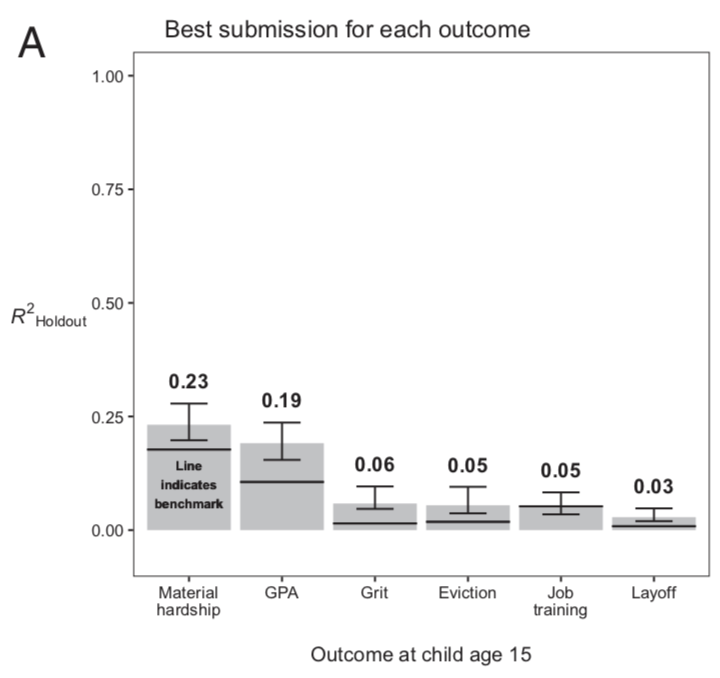
\includegraphics[width = 0.6\textwidth]{figures/salganik_measuring_2020_fig2a}
\end{center}

\end{frame}
%%%%%%%%%%%%%%%%%%%%%%%%%%%%%
\begin{frame}

\begin{center}
{\Large How can we expand our understanding?}\\ 
\vspace{0.5in}
\pause
{\Large In-depth, semi-structured interviews}
\end{center}

\vfill
Dark matter interview team: Rachel M. Brown-Weinstock, Bobbi Brashear, Kristin Catena, Susan Clampet-Lundquist, Sophie Damas, Katie Donnalley, Kaitlin Edin-Nelson, Kathryn Edin, Alexus Fraser, Sarah Gold, Ashley Hyman, Daniel Kim, Ian Lundberg, Abigail MacLean, Collin ``Ren'' MacLean, Stefanie Mavronis, Timothy Nelson, Matthew Salganik, Naomi Shifrin, and Vicki Yang.
\end{frame}
%%%%%%%%%%%%%%%%%%%%%%%%%%%
\begin{frame}

\begin{center}
{\Large Sampling}
\end{center}

\end{frame}
%%%%%%%%%%%%%%%%%%%%%%%%%%%
\begin{frame}

\begin{center}
\only<1>{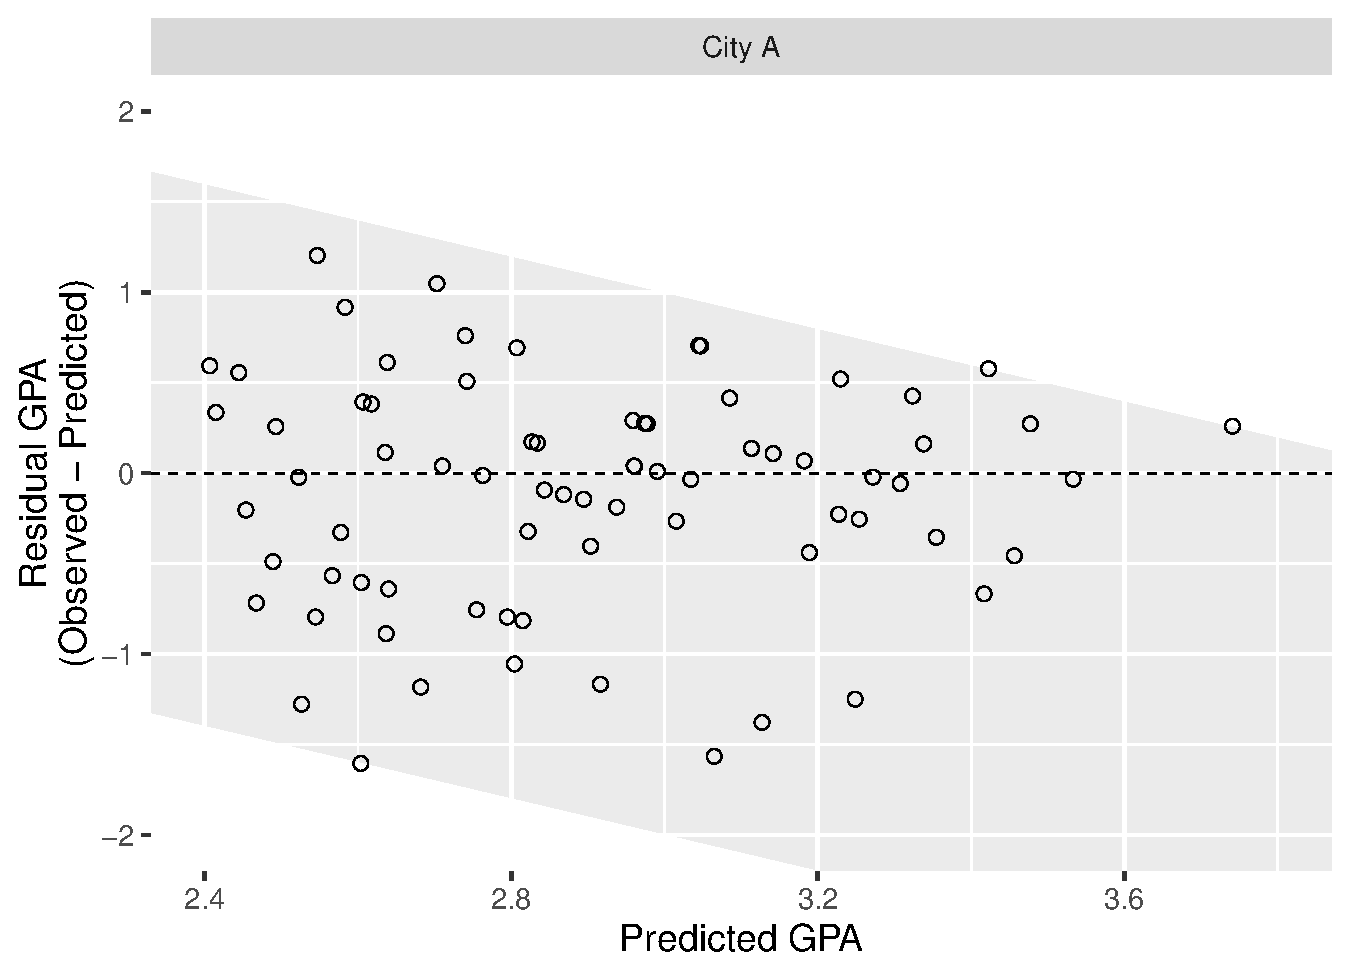
\includegraphics[width=0.8\textwidth]{figures/darkmatter_interview_sampling_talk_1}}%
\only<2>{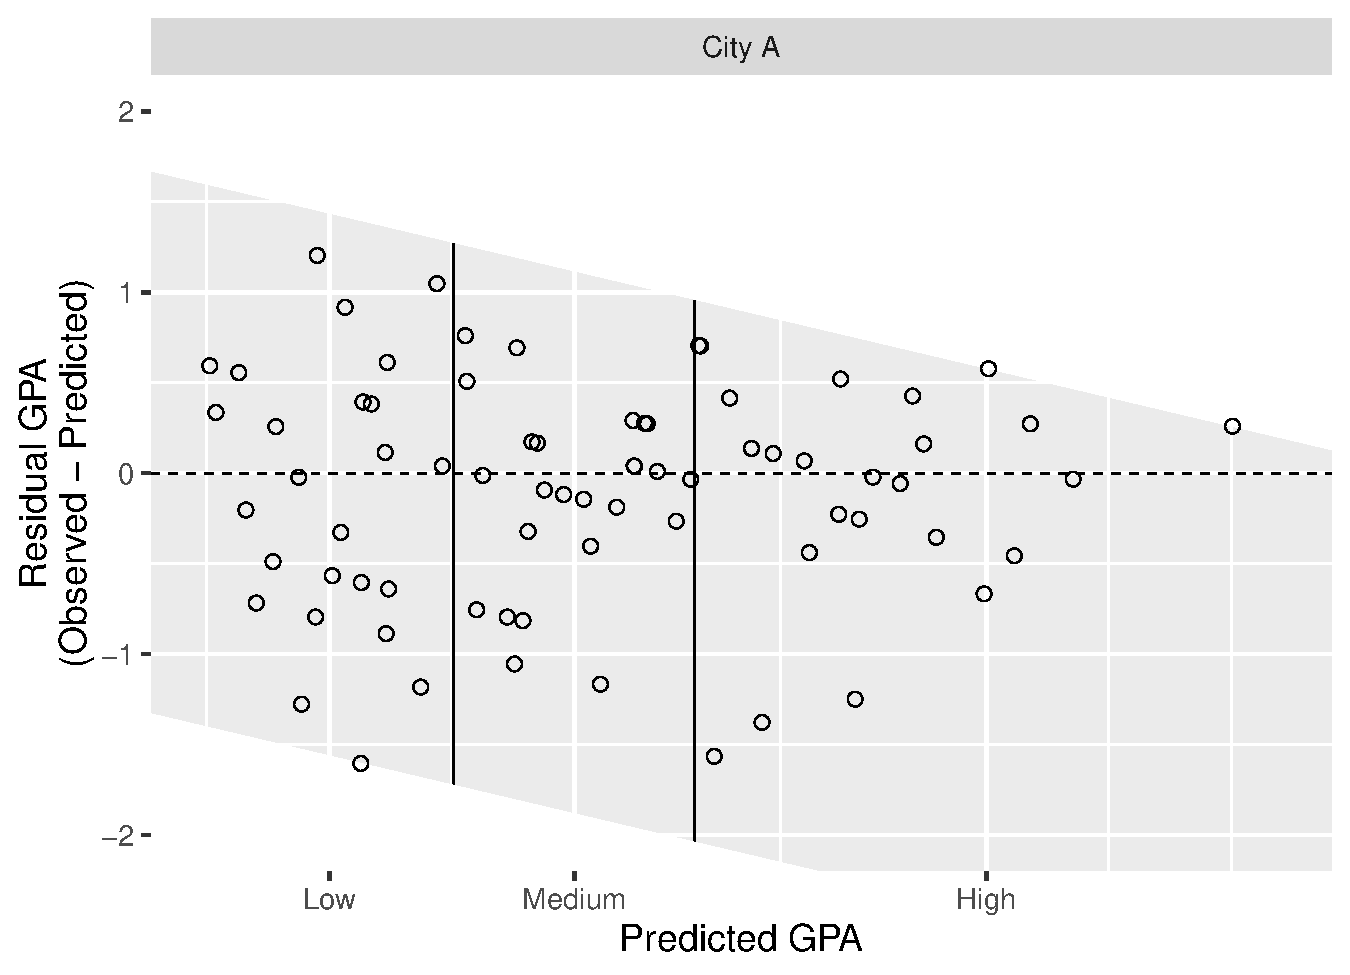
\includegraphics[width=0.8\textwidth]{figures/darkmatter_interview_sampling_talk_2}}%
\only<3>{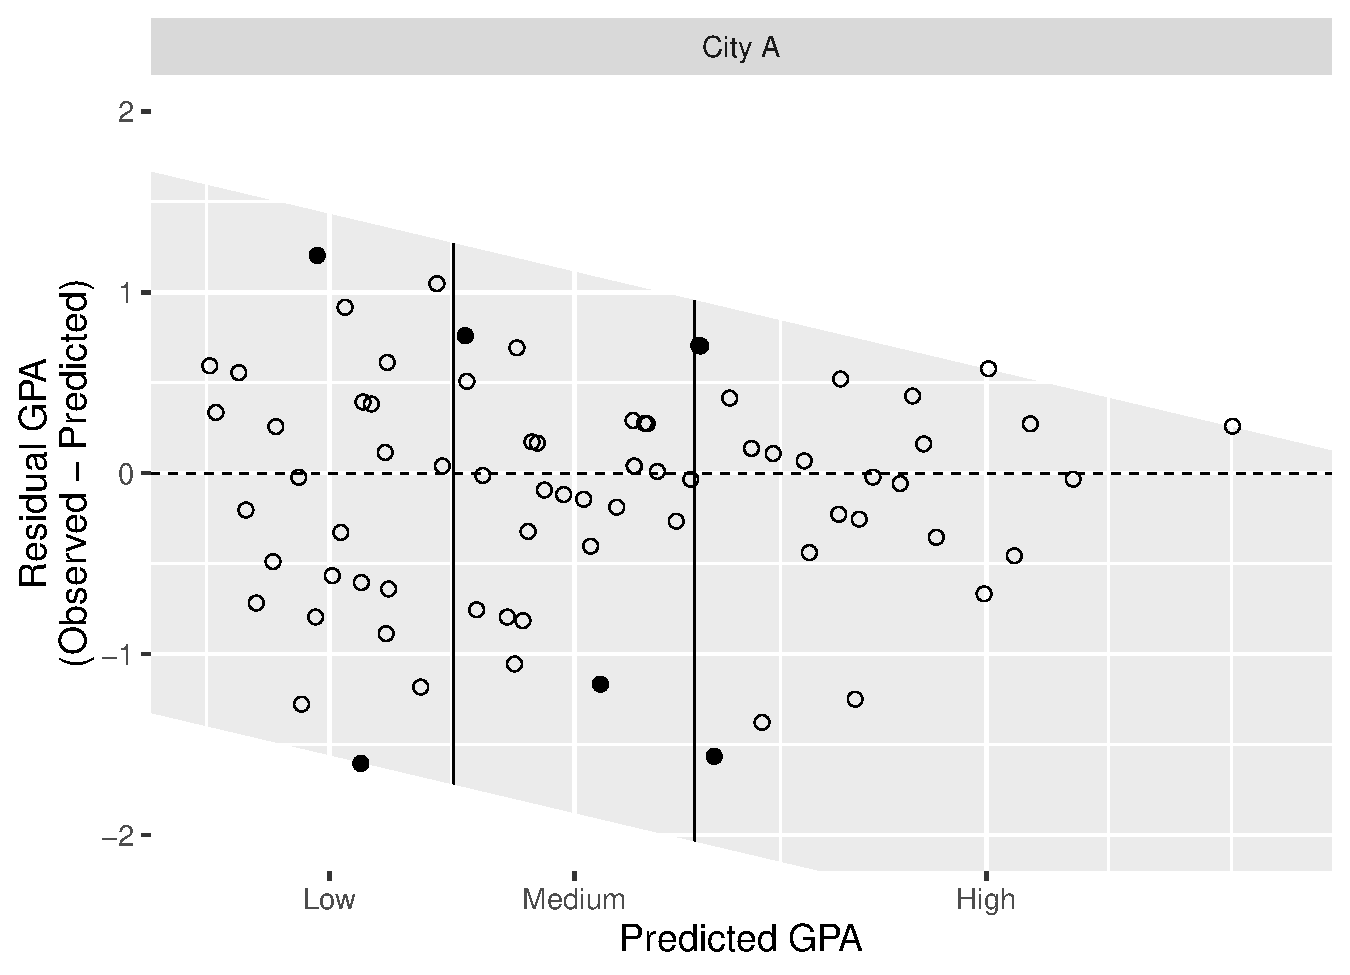
\includegraphics[width=0.8\textwidth]{figures/darkmatter_interview_sampling_talk_3}}%
\only<4>{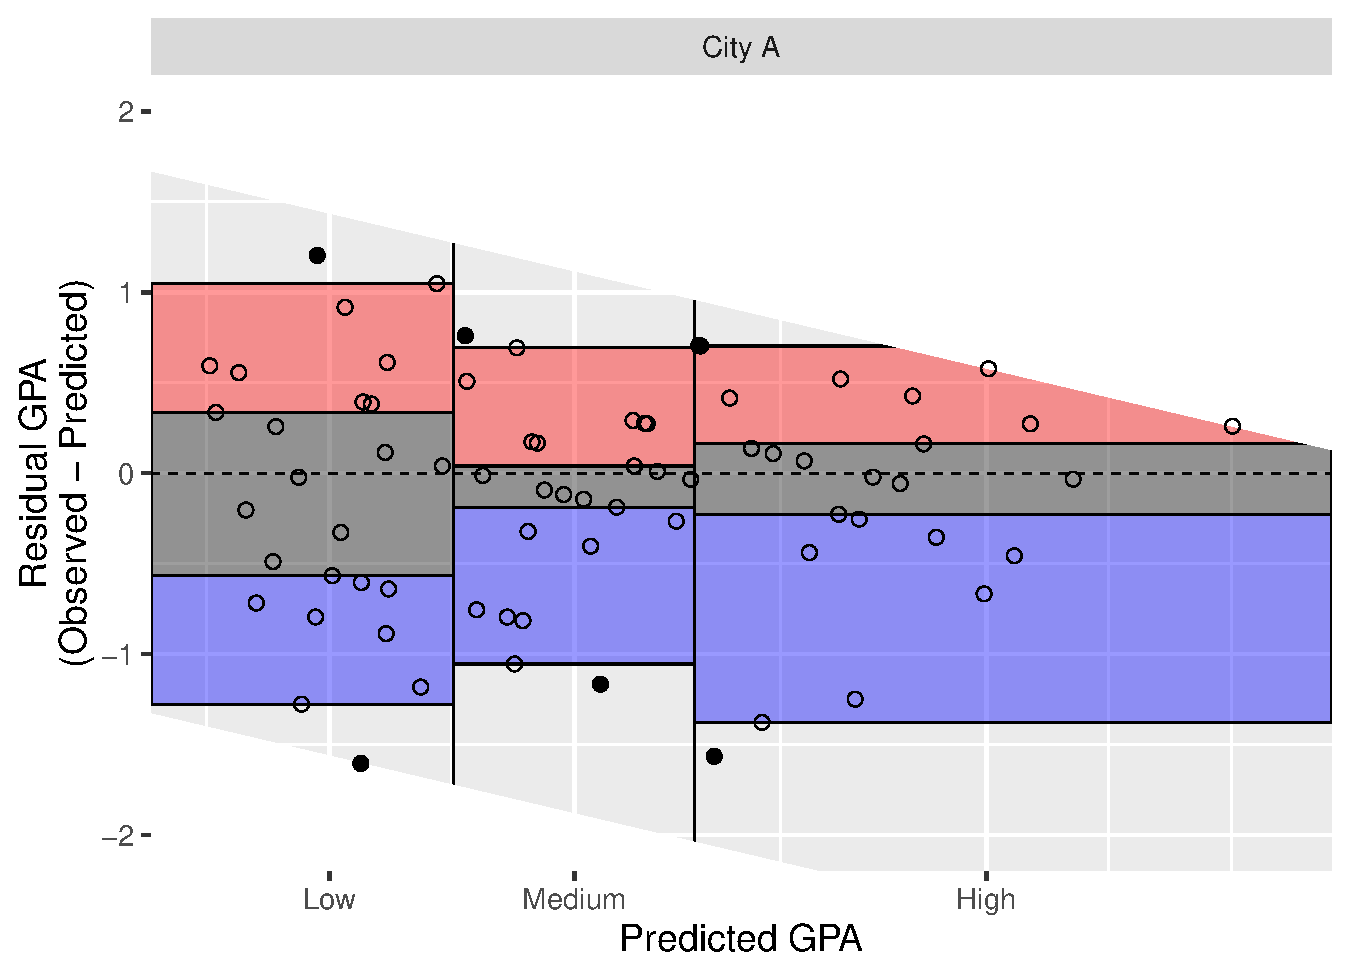
\includegraphics[width=0.8\textwidth]{figures/darkmatter_interview_sampling_talk_4}}%
\only<5>{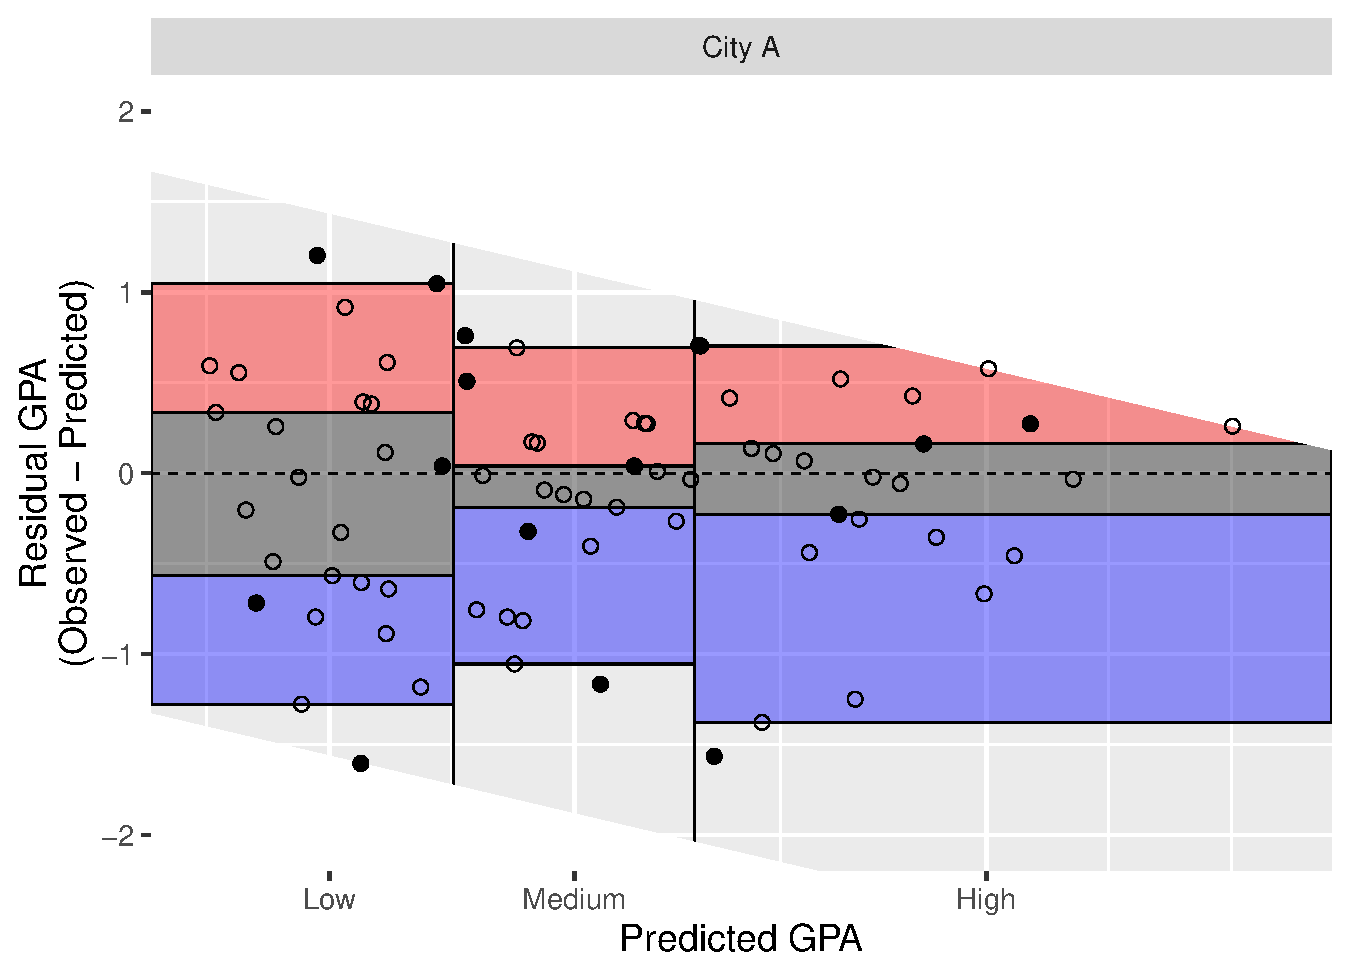
\includegraphics[width=0.8\textwidth]{figures/darkmatter_interview_sampling_talk_5}}%
\only<6>{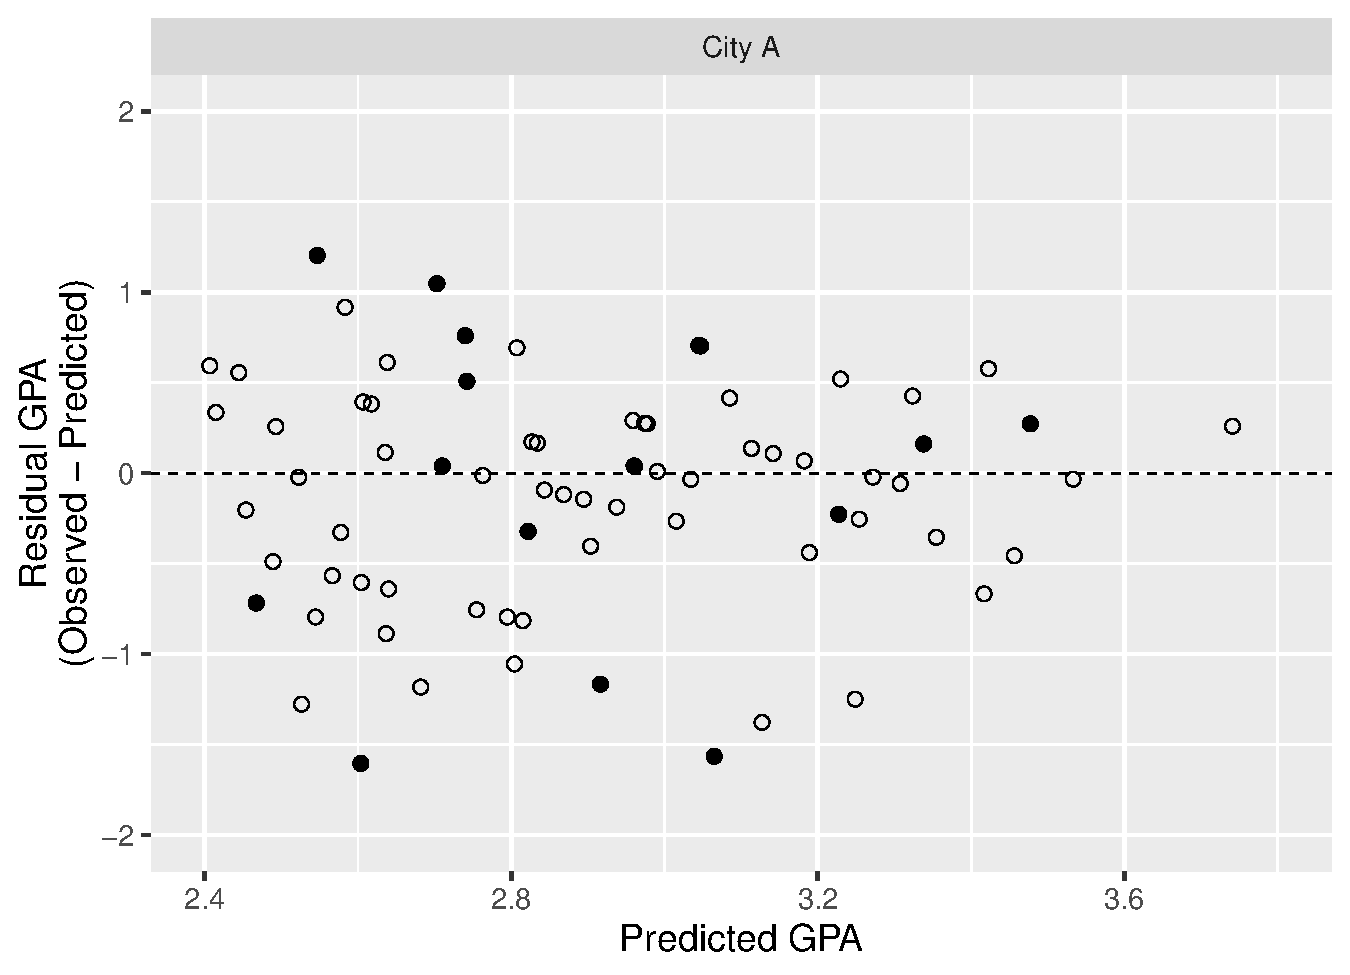
\includegraphics[width=0.8\textwidth]{figures/darkmatter_interview_sampling_talk_6}}%
\only<7>{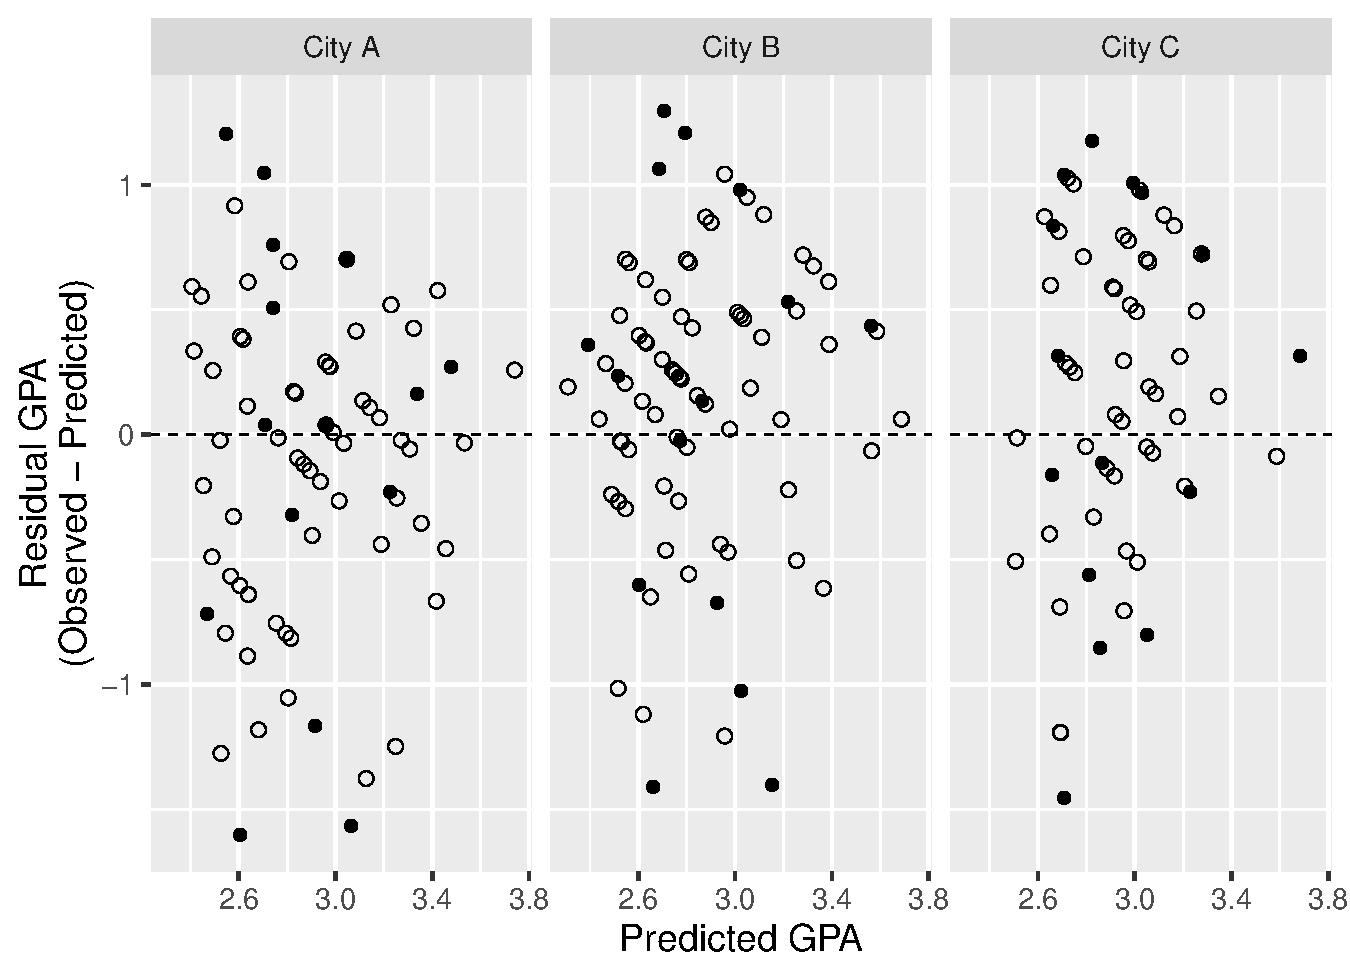
\includegraphics[width=0.8\textwidth]{figures/darkmatter_interview_sampling_talk_7}}%
\end{center}

\end{frame}
%%%%%%%%%%%%%%%%%%%%%%%%%%%
\begin{frame}

To a first approximation, we had little non-response

\end{frame}
%%%%%%%%%%%%%%%%%%%%%%%%%%%%
\begin{frame}

\begin{center}
{\Large Interviewing}
\end{center}

\end{frame}
%%%%%%%%%%%%%%%%%%%%%%%%%%
\begin{frame}

\begin{itemize}
\item Life history interviews with primary care giver and young adult and follow-up interview with young adult
\pause
\item Three key time windows: Birth - 9, 9 - 15, 15+
\pause
\item Interviews conducted in pairs, usually in the home of the respondent
\pause
\item Most interviews are 2-3 hours
\pause
\item Interviews are recorded and transcribed
\pause
\item Research protocol reviewed by the Princeton IRB
\end{itemize}

\end{frame}
%%%%%%%%%%%%%%%%%%%%%%%%%%%
\begin{frame}

\begin{columns}

\begin{column}{0.5\textwidth}
Interview guide, primary care giver
\begin{itemize}
\item Introduction
\item Education (of young adult)
\item Parenting
\item Family \& Friends (of young adult)
\item Story of Your Life as a Parent
\item Mental Health
\item Employment \& Budgets
\item Conclusion
\end{itemize}
\end{column}

\pause
\begin{column}{0.5\textwidth}
Interview guide, young adult
\begin{itemize}
\item Introduction \& Timeline
\item Education 
\item Employment
\item Family
\item Networks/Activities
\item Meaning
\item Mental Health
\item Conclusion
\end{itemize}
\end{column}

\end{columns}

\end{frame}
%%%%%%%%%%%%%%%%%%%%%%%%%%
\begin{frame}

To blind or not to blind? \pause Both

\end{frame}
%%%%%%%%%%%%%%%%%%%%%%%%%%%
\begin{frame}

\begin{center}
{\Large Analysis}
\end{center}

\end{frame}
%%%%%%%%%%%%%%%%%%%%%%%%%%%
\begin{frame}

\begin{itemize}
\item There are standard methods to analyze this kind of data, but we are not going to use them for class because 1) time constraints and 2 )they are not well suited to learn about limits to prediction 
\pause
\item Fill out the interview analysis template for family 03
\pause
\item Fill out the interview analysis template for family 42
\end{itemize}

\end{frame}
%%%%%%%%%%%%%%%%%%%%%%%%%%%
\begin{frame}

\begin{center}
{\Large Case selection for this class}
\end{center}

\end{frame}
%%%%%%%%%%%%%%%%%%%%%%%%%%%%%%
\begin{frame}

\begin{itemize}
\item I did the interviews with one of these families, and I found it very enlightening
\pause
\item Looked for a shorter one to pair with it; shortest one was translated from Spanish, next shortest was similar to the one I did, next shortest seemed quite different
\end{itemize}

\end{frame}
%%%%%%%%%%%%%%%%%%%%%%%%%%%%%%
\begin{frame}

\begin{center}
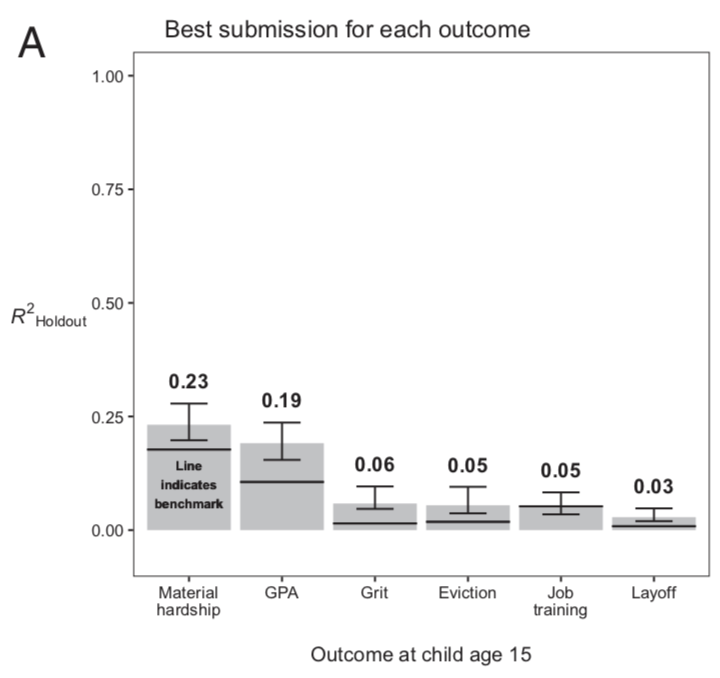
\includegraphics[width = 0.6\textwidth]{figures/salganik_measuring_2020_fig2a}
\end{center}

\end{frame}
%%%%%%%%%%%%%%%%%%%%%%%%%%%%%
\frame{\titlepage}


\end{document}
